\documentclass[a4paper, 11pt]{article}

\usepackage[T2A]{fontenc}
\usepackage[utf8]{inputenc}
\usepackage[english, russian]{babel}
\usepackage{amsmath}
\usepackage{graphicx}
\usepackage{subcaption}
\usepackage{float}
\usepackage{tabularx}
\usepackage{amsmath,booktabs}
\usepackage{array}
\righthyphenmin=2
\usepackage[left=20mm, top=15mm, right=15mm, bottom=15mm, nohead, footskip=10mm]{geometry} % настройки полей документа
\usepackage{caption}
\DeclareCaptionLabelSeparator{dash}{ – }
\captionsetup{justification=centering,labelsep=dash}
\newcommand\tline[2]{$\underset{\text{#1}}{\text{\underline{\hspace{#2}}}}$}
\captionsetup[table]{justification=justified,singlelinecheck=false}
\begin{document} 

% НАЧАЛО ДОКУМЕНТА
%_______________
	\begin{titlepage}
		\centering
		{\fontsize{12pt}{5cm}\selectfont \bfseries Министерство образования и науки Российской Федерации} \\ \vspace{0.5cm}
		{\fontsize{7pt}{5cm}\selectfont ФЕДЕРАЛЬНОЕ ГОСУДАРСТВЕННОЕ АВТОНОМНОЕ ОБРАЗОВАТЕЛЬНОЕ УЧРЕЖДЕНИЕ ВЫСШЕГО ПРОФЕССИОНАЛЬНОГО ОБРАЗОВАНИЯ} \\ 
		\vspace{1cm}
		{\fontsize{12pt}{5cm}\selectfont \bfseries САНКТ-ПЕТЕРБУРГСКИЙ УНИВЕРСИТЕТ ИНФОРМАЦИОННЫХ ТЕХНОЛОГИЙ, МЕХАНИКИ И ОПТИКИ} \\ \vspace{1.5cm}
		
		{\fontsize{14pt}{5cm}\selectfont Кафедра \hspace{1cm} \underline{Систем Управления и Информатики}  \hspace{1cm} Группа \underline{Р3340}} \\ 
		\vspace{2cm}
		
		{\fontsize{20pt}{5cm}\selectfont \bfseries Лабораторная работа №7} \\
		{\fontsize{20pt}{5cm}\selectfont \bfseries “Анализ точности систем управления”} \\
		{\fontsize{14pt}{5cm}\selectfont Вариант - 02} \\
		\vspace{1.5cm}
		
		\flushleft
		
		{Выполнил \hspace{0.5cm} \tline{(фамилия, и.о.)}{10cm} (подпись)} \\
		\vspace{2cm}
		
		{Проверил \hspace{0.5cm} \tline{(фамилия, и.о.)}{10cm} (подпись)} \\
		\vspace{5cm}
		
		"\underline{\hspace{0.4cm}}"\hspace{0.1cm}\underline{\hspace{1.5cm}}\hspace{0.1cm}20\underline{\hspace{0.4cm}}г. \hspace{2cm} Санкт-Петербург, \hspace{2cm} 20\underline{\hspace{0.4cm}}г. \\ \vspace{1cm}
		
		Работа выполнена с оценкой \hspace{0.5cm} \underline{\hspace{10cm}} \\ 
		\vspace{1cm}
		Дата защиты "\underline{\hspace{0.4cm}}"\hspace{0.1cm}\underline{\hspace{1.5cm}}\hspace{0.1cm}20\underline{\hspace{0.4cm}}г.
		
	\end{titlepage}
%_______________	
\section*{Цель работы}Исследование точностных свойств систем управления.

\section*{Исходные данные}

\begin{tabular}{cccc}
	& \multicolumn{3}{c}{Параметры сигнала задания} \\
	\raisebox{1.5ex}[0cm][0cm]{Передаточная функция $W(s)$}
	& $g = A$ & $g = Vt$ & $g = at^2$ \\
	\hline\\
	$\frac{3} {2.5s+1}$ & $2$ & $2t$ & $0.5t^2$ \\
\end{tabular}

\newpage

\begin{center}
\section{Исследование системы с астатизмом нулевого порядка}
\end{center}
\subsection{Стационарный режим работы системы} На рисунке 1 представлена схема моделирования системы с астатизмом нулевого порядка при входном воздействии g = 2, также на рисунках 2 и 3 представлены графики переходного процесса и ошибки при разных коэффициентах.

\begin{figure}[h]
    \center{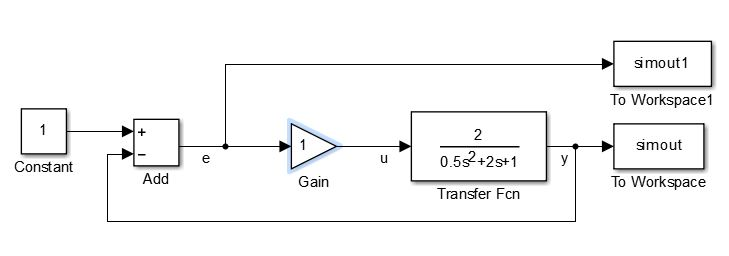
\includegraphics[width=1\linewidth]{1}}
    \caption{Система с астатизмом нулевого порядка}
    \label{one}
\end{figure}

\begin{figure}[h!]
    \center{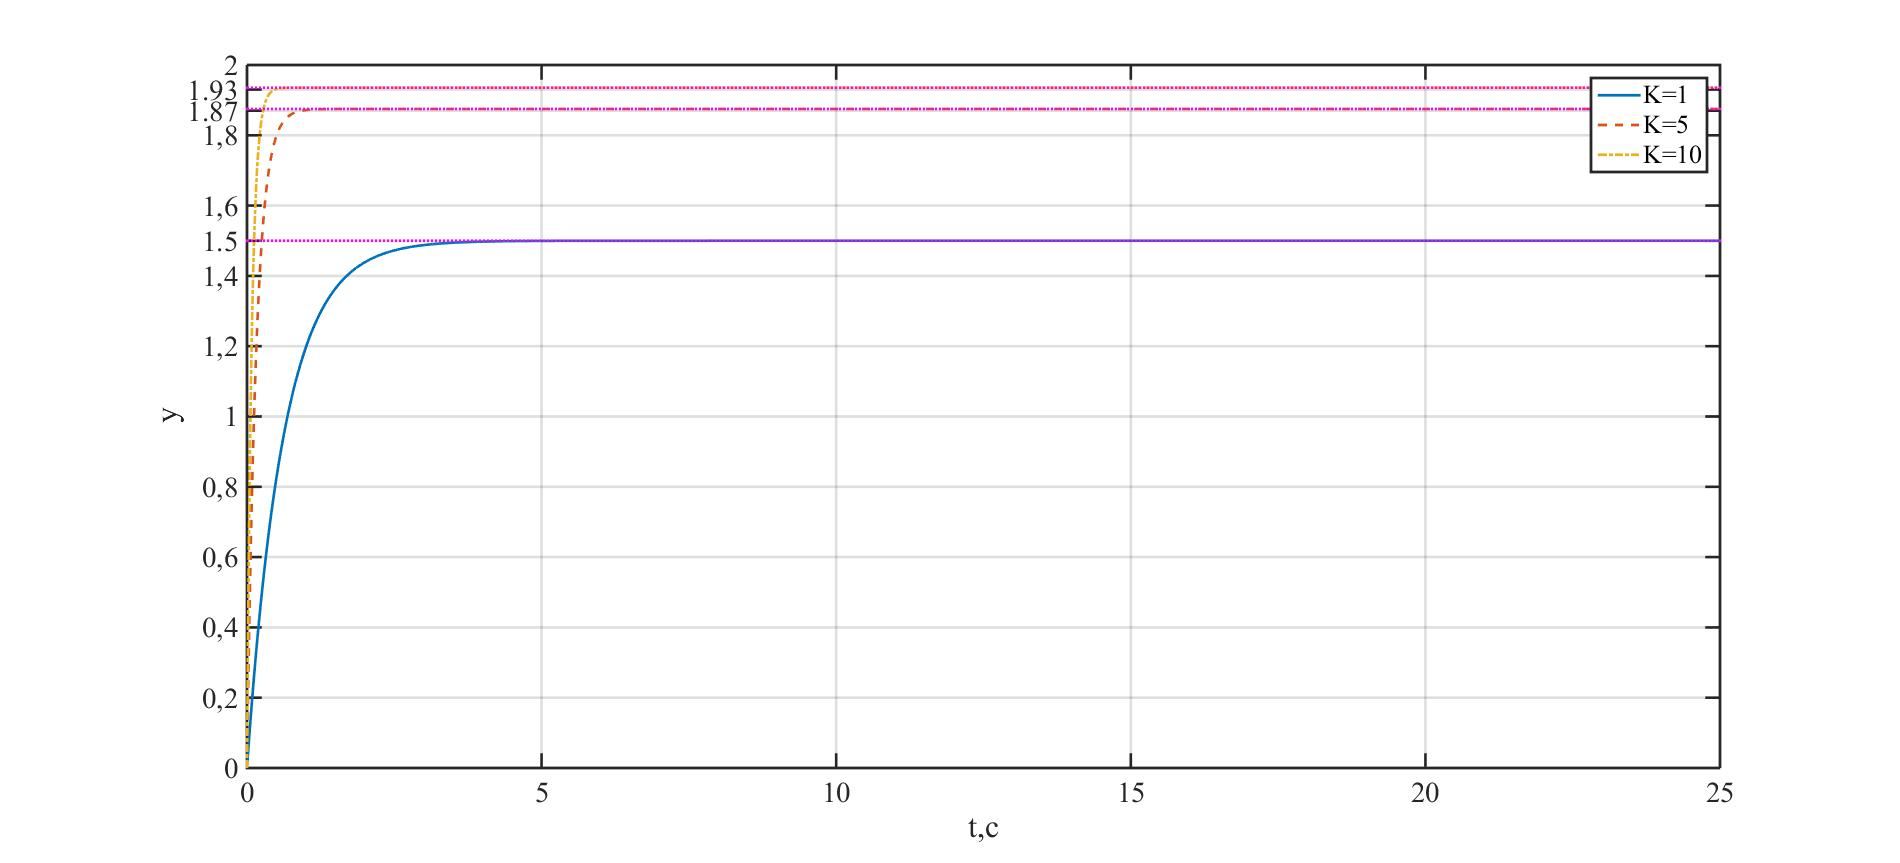
\includegraphics[width=1\linewidth]{1/a2y}}
    \caption{График переходного процесса}
    \label{two}
\end{figure}



\begin{figure}[h!]
    \center{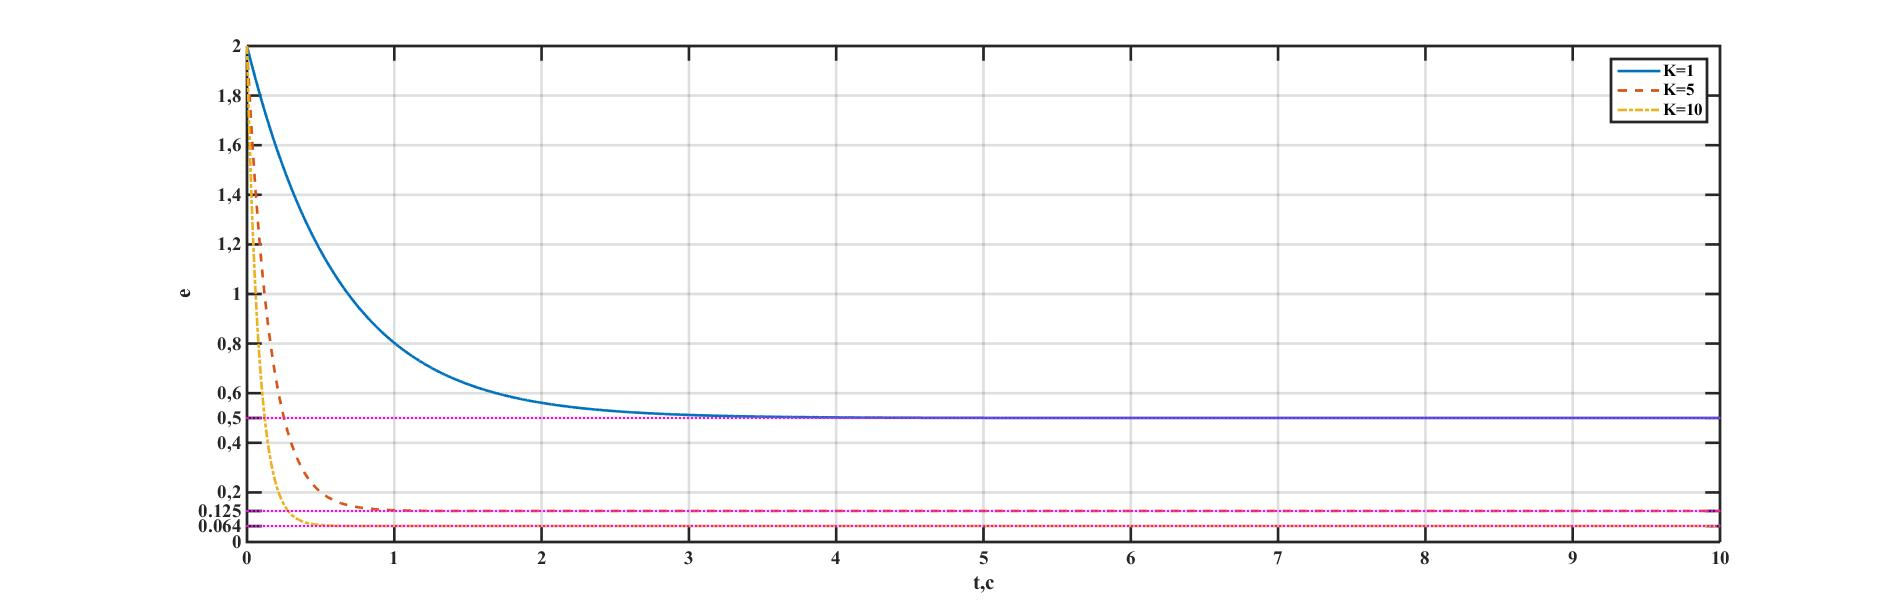
\includegraphics[width=1\linewidth]{1/a2e}}
    \caption{График ошибки переходного процесса}
    \label{tree}
\end{figure}


Предельное значение ошибки рассчитывается по формуле:

\begin{equation}
	\varepsilon = \lim_{s\to 0}{\Phi_e(s)}g =\frac {A}{1+3k}
\end{equation}

На таблице 1 рассчитаны аналитическим методом ошибки переходного процесса.

\newpage

\begin{table}[h]
		\caption{Зависимость коэффициента от ошибки}
		\begin{tabular}{|c|c|c|c|}
			\hline
			K & 1 & 5 & 10 \\
			\hline
			$\varepsilon$ & 0.5 & 0.125 & 0.064 \\
			\hline     
		\end{tabular}
		
		\label{tab:my_label}
\end{table}

Значения $\varepsilon$ полученные аналитическим методом полностью совпадают с установившимися значениями ошибки на графике.

%_______________ПРИ g(t)=Vt
\subsection{Работа с постоянной скоростью} g(t) = Vt – движение с постоянной скоростью. V = 2\\На рисунках 4 и 5 представлены гафики переходного процесса сигнала и ошибки.


\begin{figure}[h!]
    \center{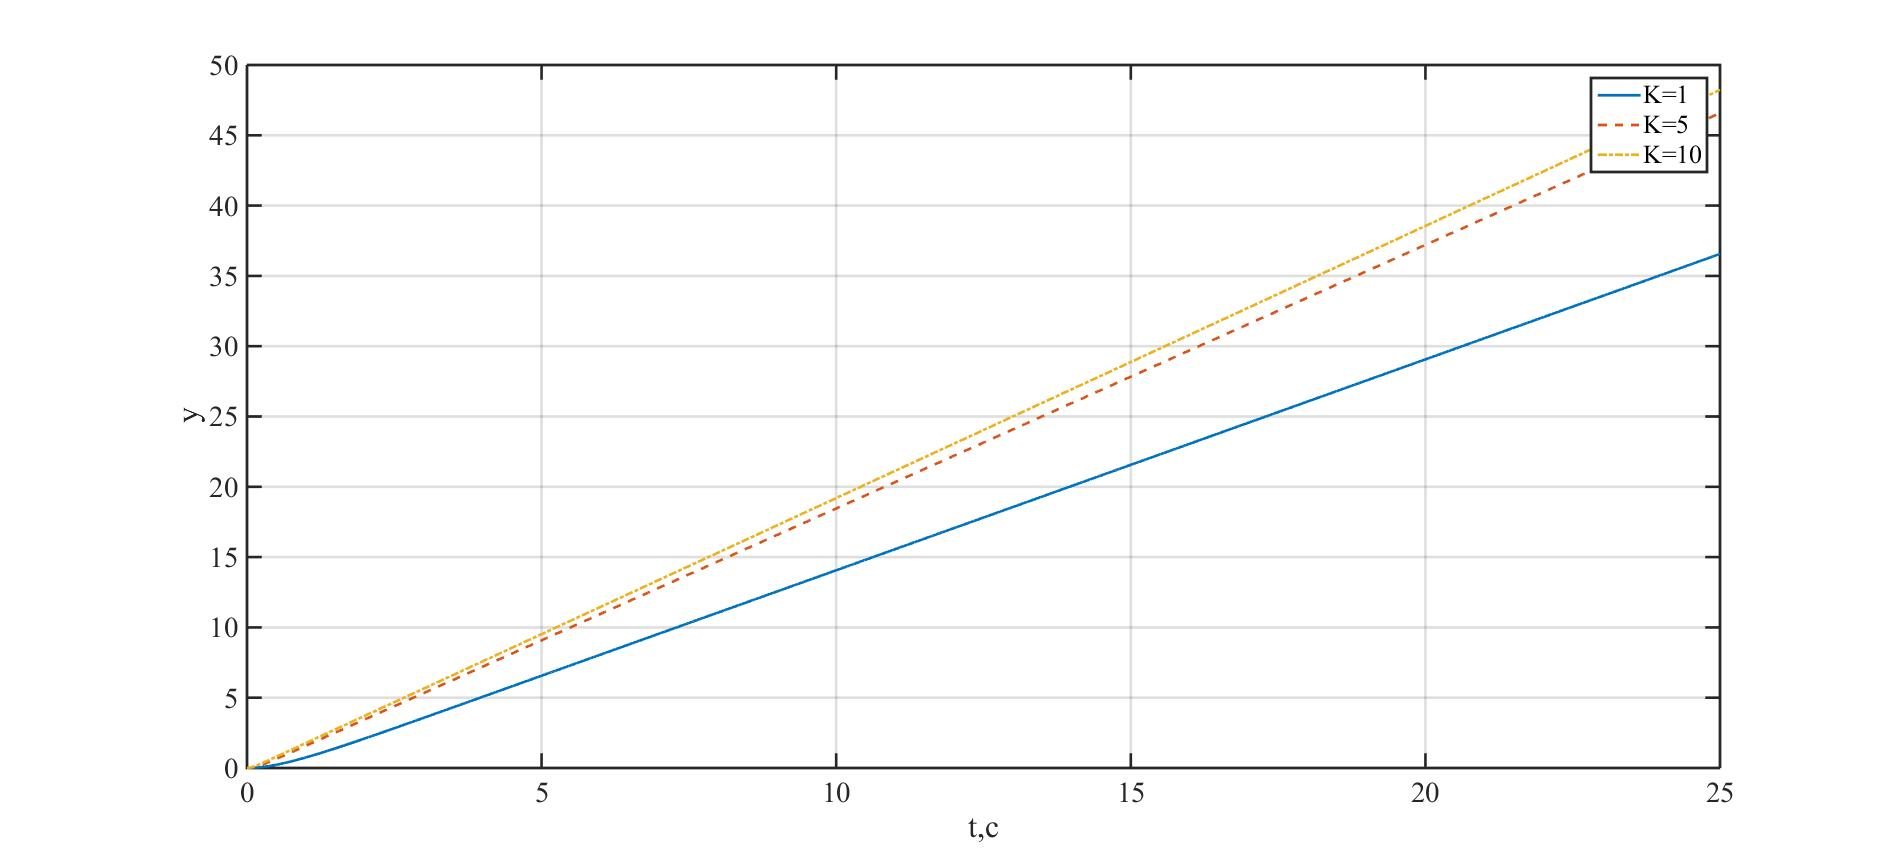
\includegraphics[width=1\linewidth]{1/v2ty}}
    \caption{График переходного процесса}
    \label{four}
\end{figure}
\begin{figure}[h!]
    \center{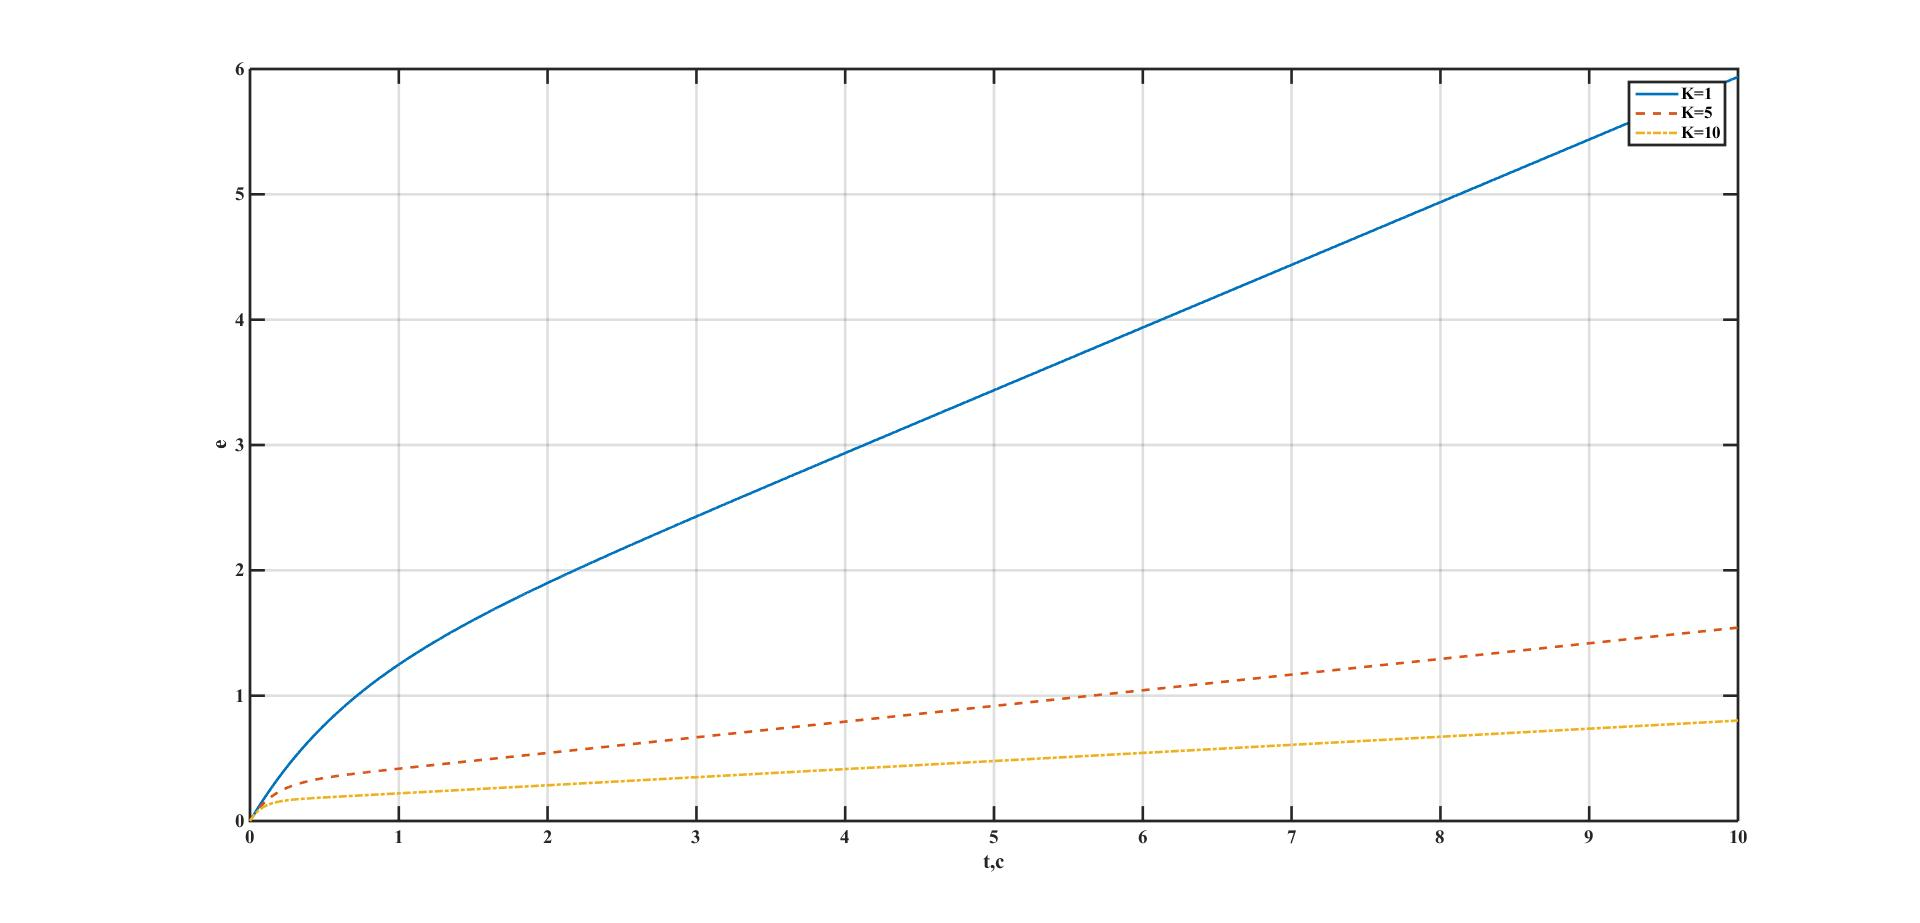
\includegraphics[width=1\linewidth]{1/v2te}}
    \caption{График ошибки переходного процесса}
    \label{tree}
\end{figure}

Аналитический расчет установившихся значений ошибки:\\
$\varepsilon_y(t)=\lim_{s\to0}s\frac{1}{1+W(s)}\frac{V}{s^2}=\lim_{s\to0}\frac{1}{1+k}\frac{V}{s}=\infty$

Во всех случаях $\varepsilon\to\infty$ 

%___________________ВТОРАЯ ЧАСТЬ____________________
\newpage

\begin{center}
\section{Исследование системы с астатизмом первого порядка}
\end{center}
\subsection{Стационарный режим работы}На рисунке 6 представлена схема моделирования системы с астатизмом первого порядка при входном воздействии g = 2, также на рисунках 7 и 8 представлены графики переходного процесса и ошибки при разных коэффициентах.\\
Исследуемая система: \large{$W(s)=\frac{3}{2.5s+1}$}


\begin{figure}[h!]
    \center{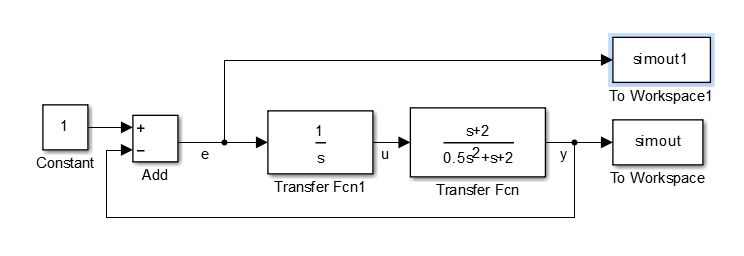
\includegraphics[width=1\linewidth]{2}}
    \caption{Система с астатизмом первого порядка}
    \label{one}
\end{figure}
%___________Поехали а

\begin{figure}[h!]
    \center{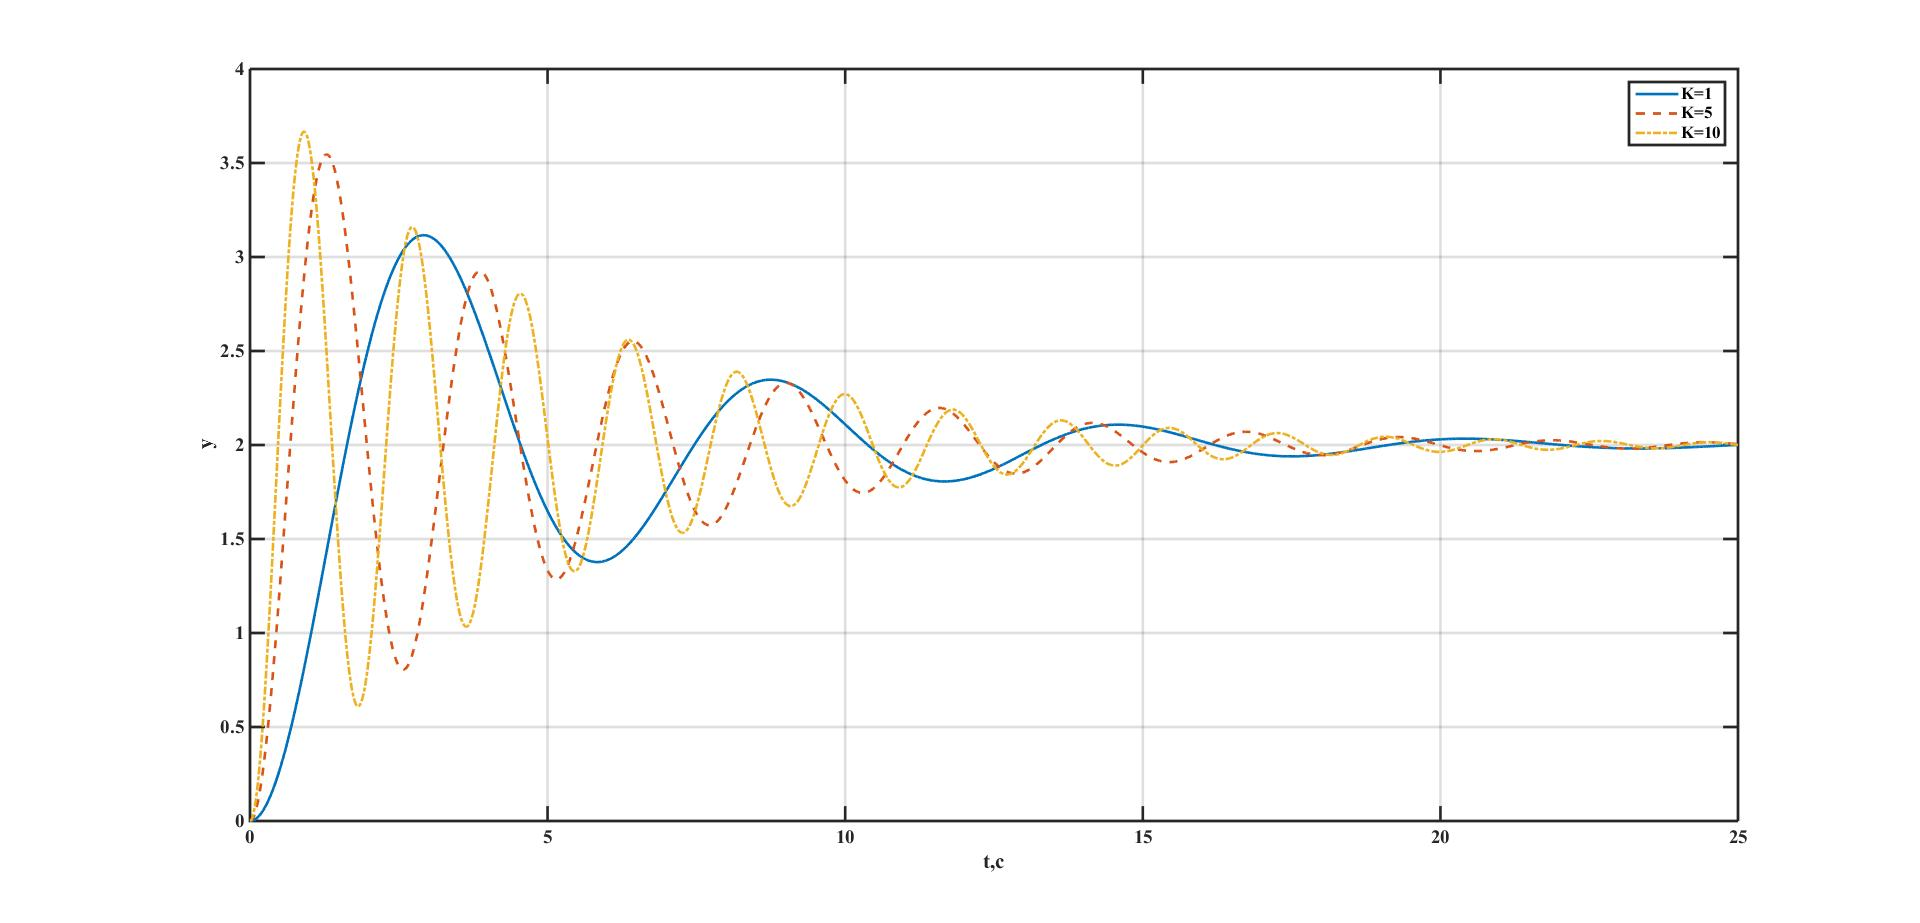
\includegraphics[width=1\linewidth]{2/1a2y}}
    \caption{График переходного процесса}
    \label{two}
\end{figure}

\newpage

\begin{figure}[h!]
    \center{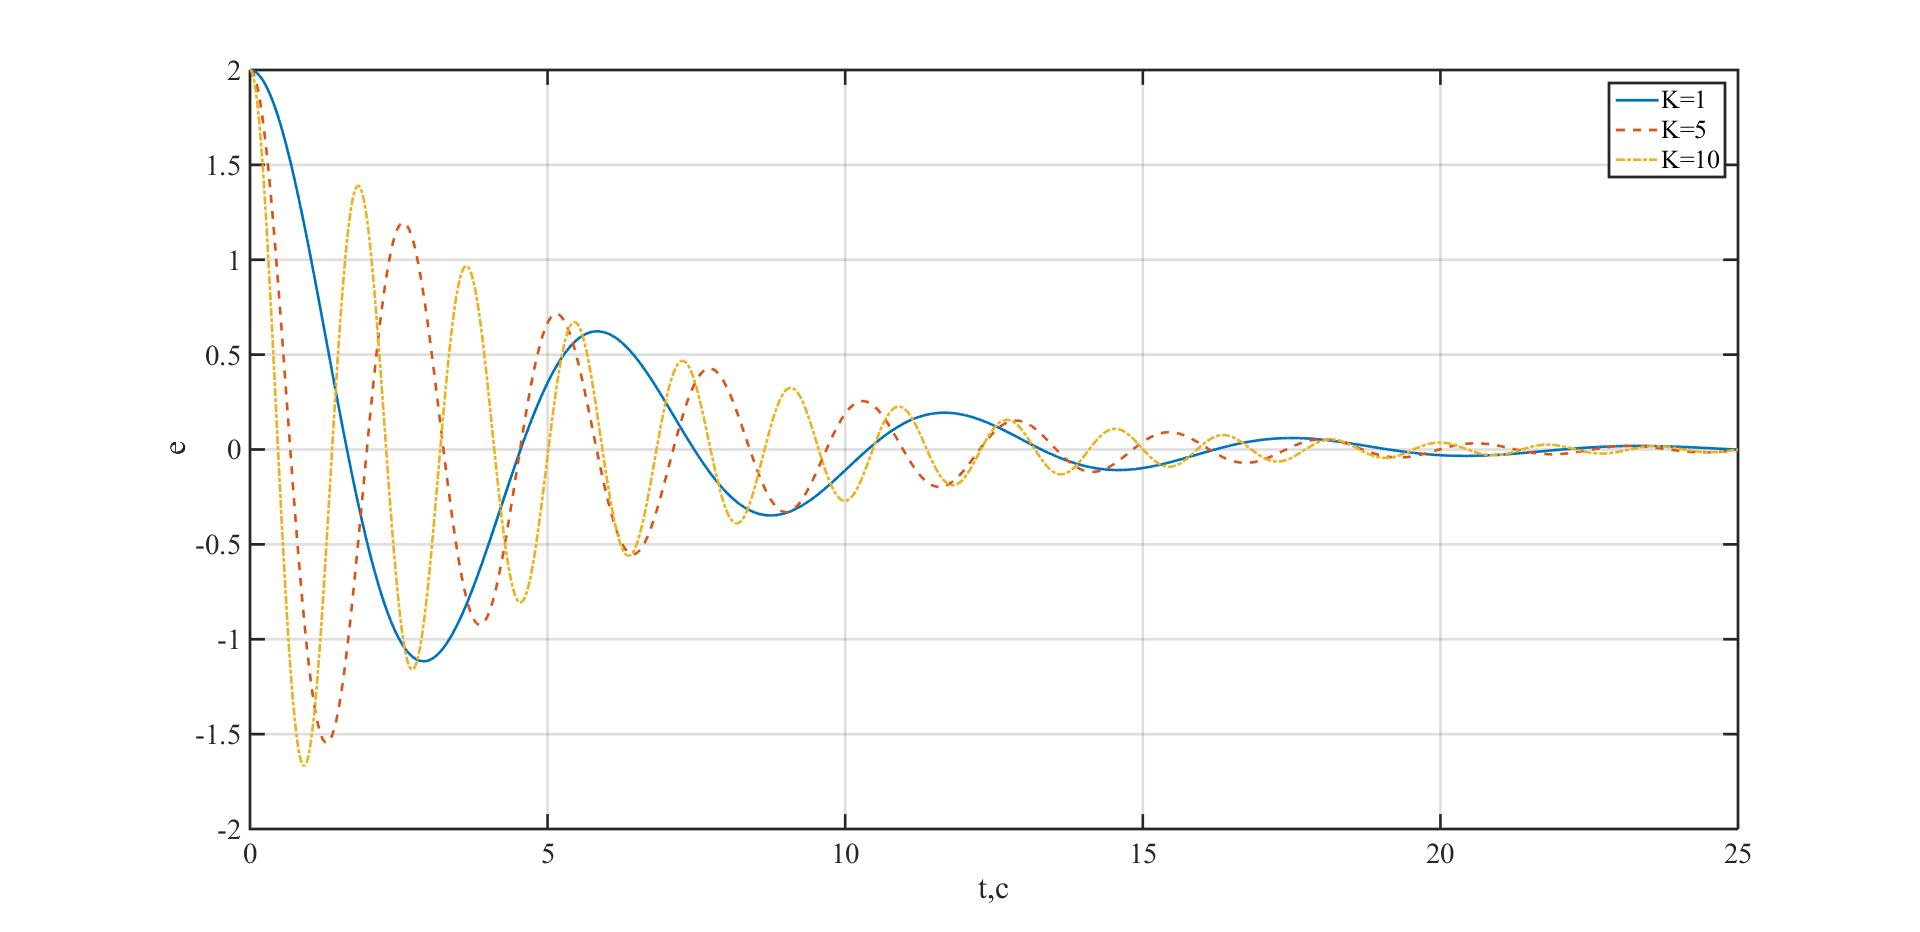
\includegraphics[width=1\linewidth]{2/1a2e}}
    \caption{График ошибки переходного процесса}
    \label{tree}
\end{figure}

Из графика видно, что предельное значение установившихся ошибок $\varepsilon_y(t)=0$. Это значение подтверждается аналитическим расчетом: $\varepsilon_y(t)=\lim_{s\to0}\frac{s}{s+k}A=0$\\


%___________________Б-часть второго параграфа
\subsection{Работа с постоянной скоростью} g(t) = Vt – движение с постоянной скоростью. V = 2. На рисунках 9 и 10 представлены гафики переходного процесса сигнала и ошибки.


\begin{figure}[h!]
    \center{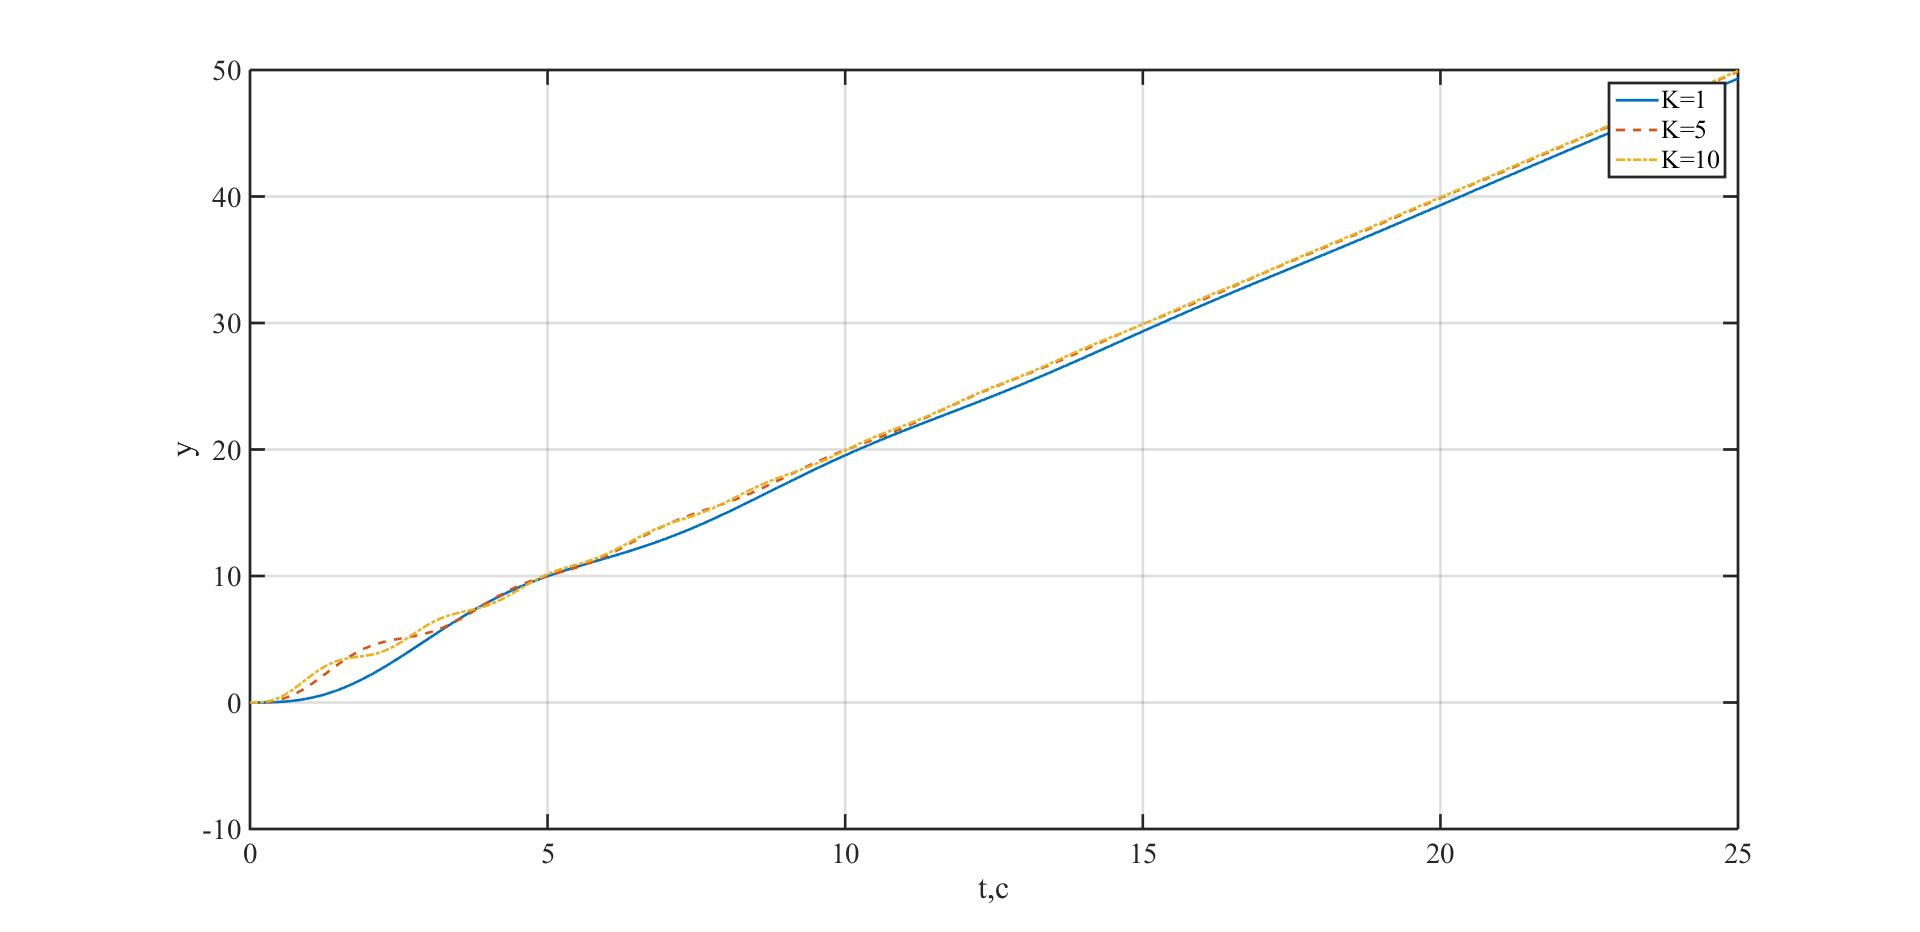
\includegraphics[width=1\linewidth]{2/1v2ty}}
    \caption{График переходного процесса}
    \label{two}
\end{figure}

\newpage

\begin{figure}[h!]
    \center{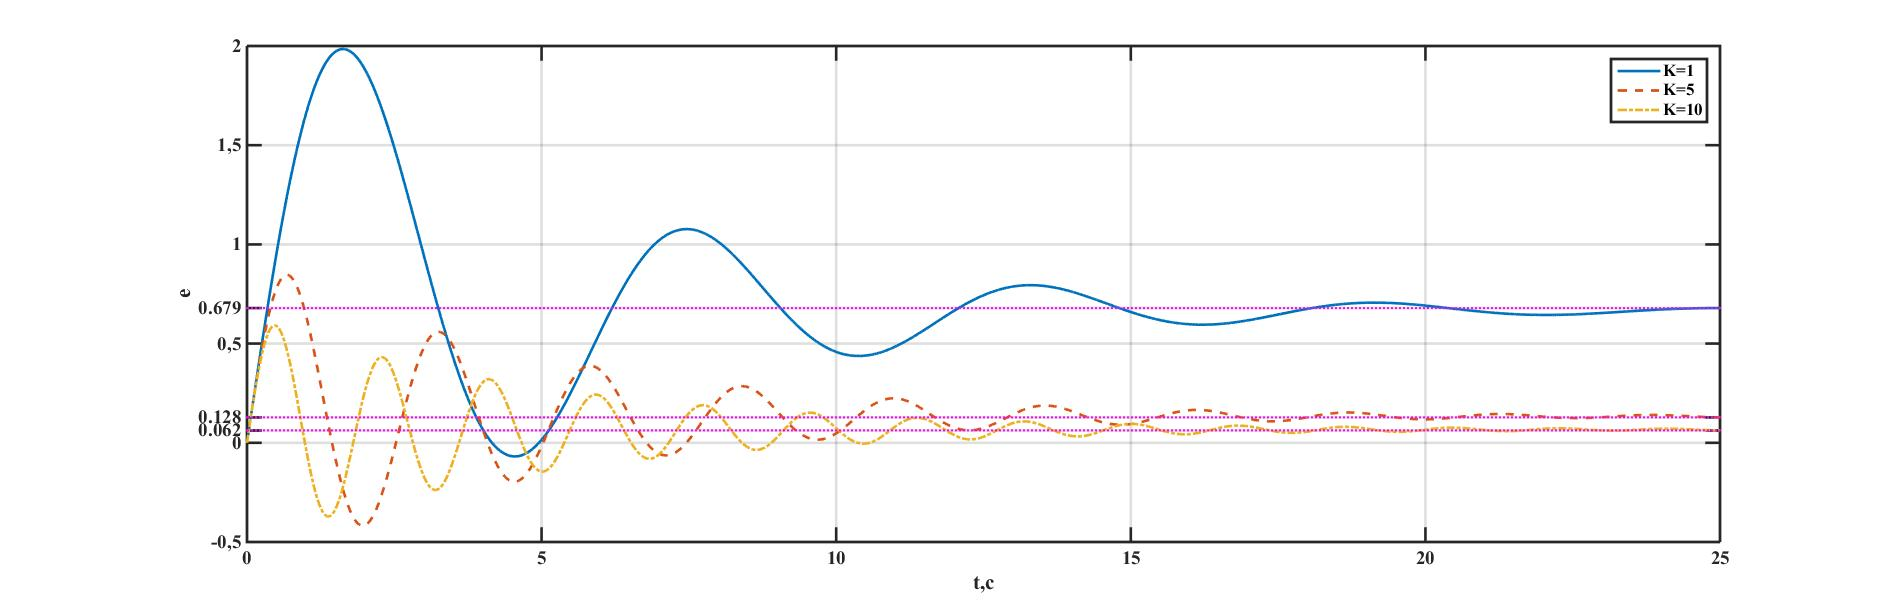
\includegraphics[width=1\linewidth]{2/1v2te}}
    \caption{График ошибки переходного процесса}
    \label{tree}
\end{figure}

\begin{equation}
	\varepsilon_y(t)=\lim_{s\to0}\frac{s}{s+k}V=\frac{V}{3k}
\end{equation}

На таблице 1 рассчитаны аналитическим методом ошибки переходного процесса.

\begin{table}[h]
    \caption{Зависимость коэффициента от ошибки}
    \begin{tabular}{|c|c|c|c|}
    \hline
         K & 1 & 5 & 10 \\
         \hline
         $\varepsilon$ & 0.666 & 0.133 & 0.066 \\
    \hline     
    \end{tabular}    
    \label{tab:two}
\end{table}

Значения $\varepsilon$ полученные аналитическим методом почти совпадают с установившимися значениями ошибки на графике.\\


%_______________В в параграфе 2
\subsection{Движение с постоянным искорением} $g(t)=at^2/2$ – движение с постоянным ускорением. a = 0.5. На рисунках 11 и 12 представлены гафики переходного процесса сигнала и ошибки.

\begin{figure}[h!]
    \center{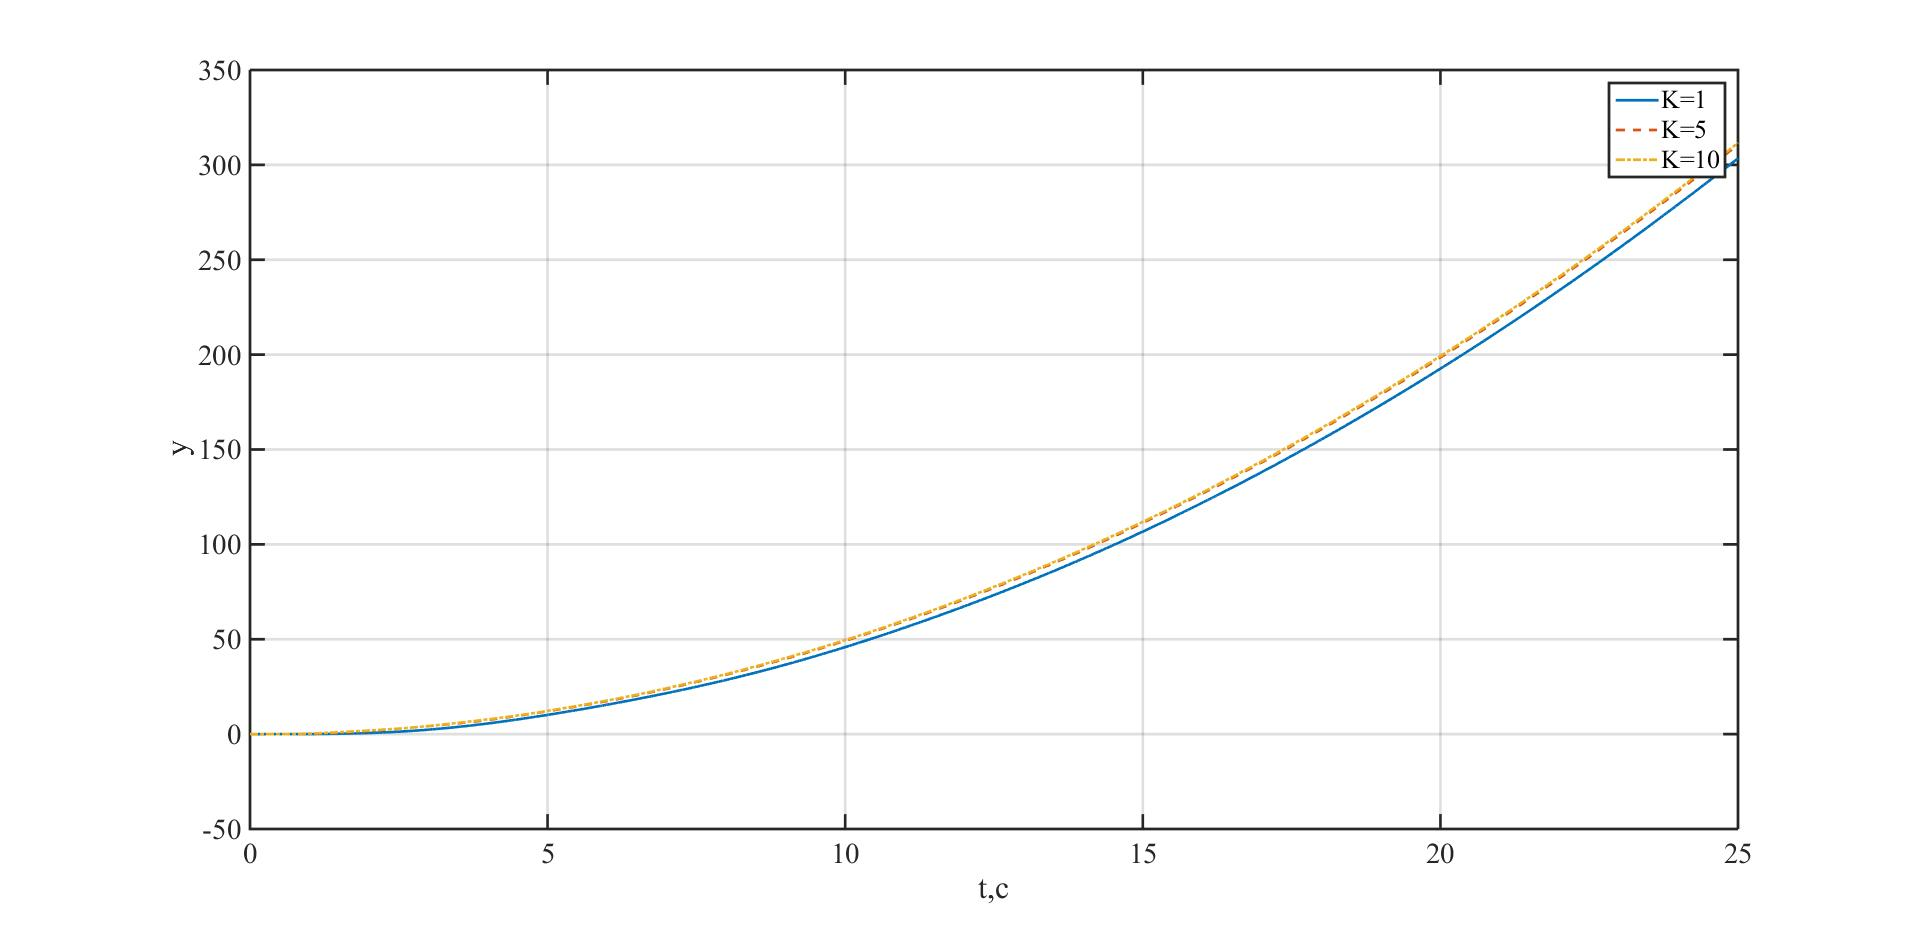
\includegraphics[width=1\linewidth]{2/1g05ty}}
    \caption{График переходного процесса}
    \label{two}
\end{figure}

\newpage

\begin{figure}[h!]
    \center{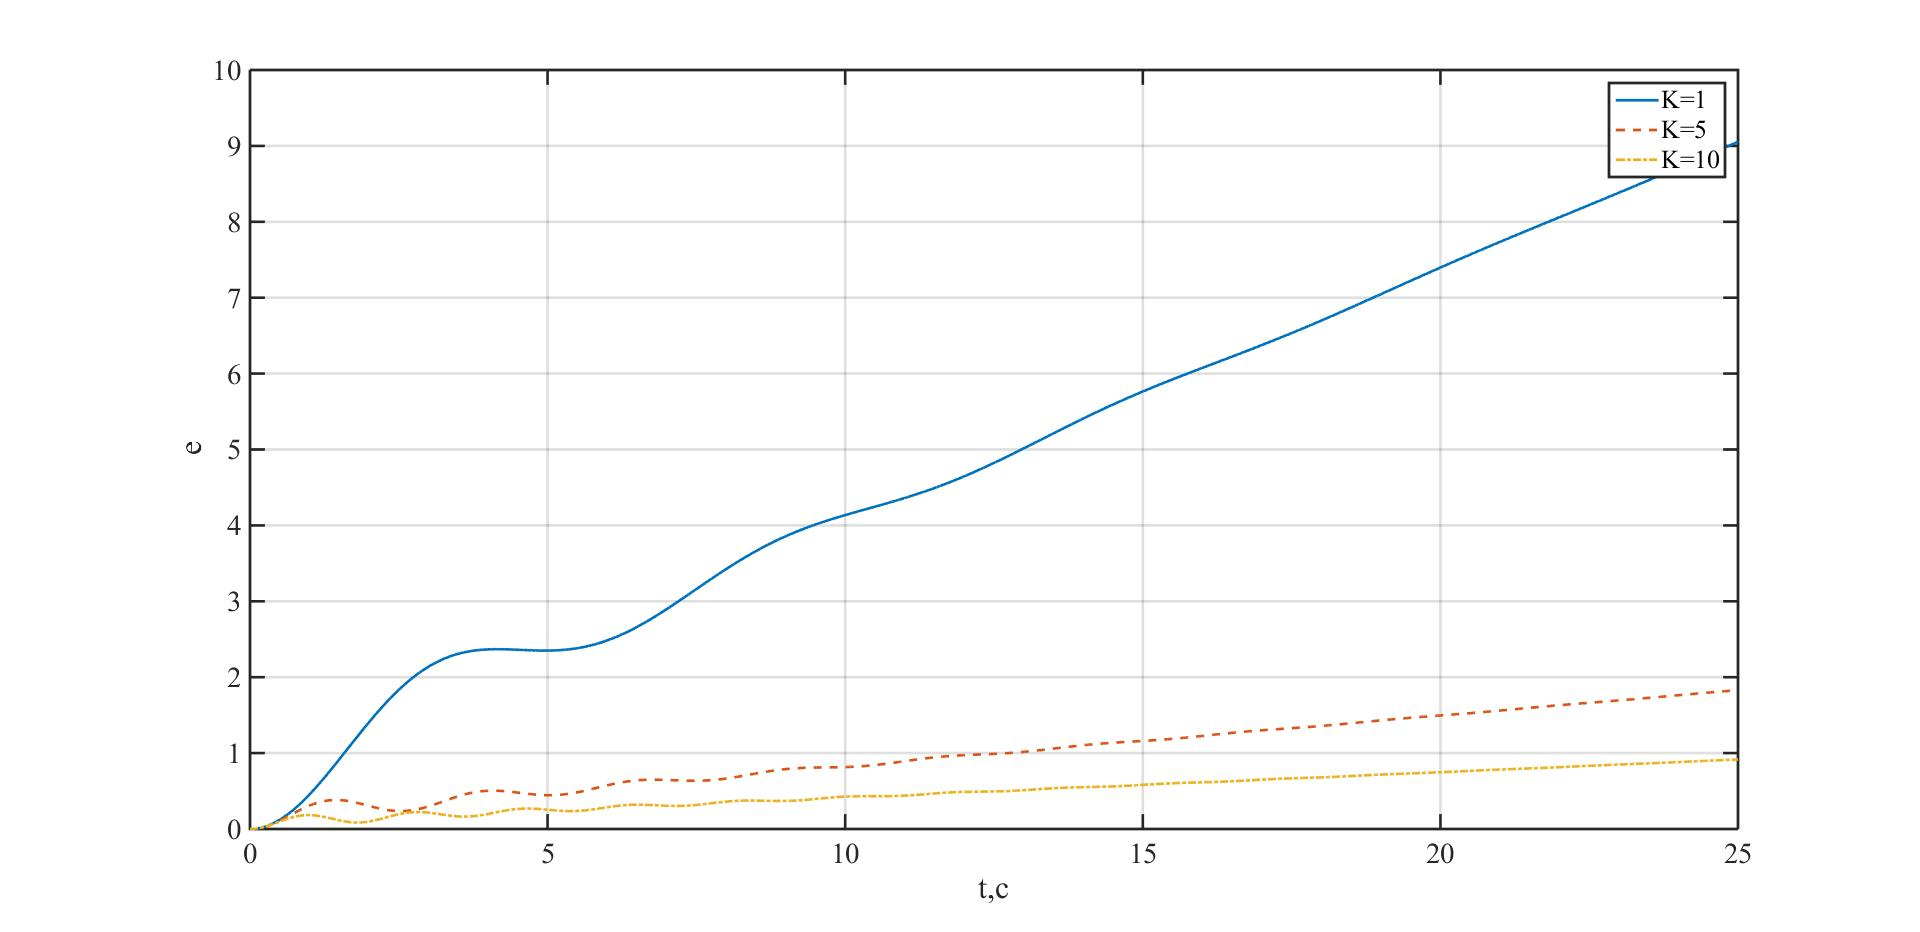
\includegraphics[width=1\linewidth]{2/1g05te}}
    \caption{График ошибки переходного процесса}
    \label{o:tree}
\end{figure}

\newpage

%ТРЕТИЙ ПАРАГРАФ______________!!!!!!!!!!!!!!!!!
\begin{center}
\section{Исследование влияния внешних возмущений}
\end{center}
На рисунке 13 представлена схема моделирования влияния внешних возмущений, также на рисунках 14, 15, 16 и 17 представлены графики переходного процесса и ошибки при различных значениях шумов $f_1=0.5,  f_2=0.5$

\begin{figure}[h!]
    \center{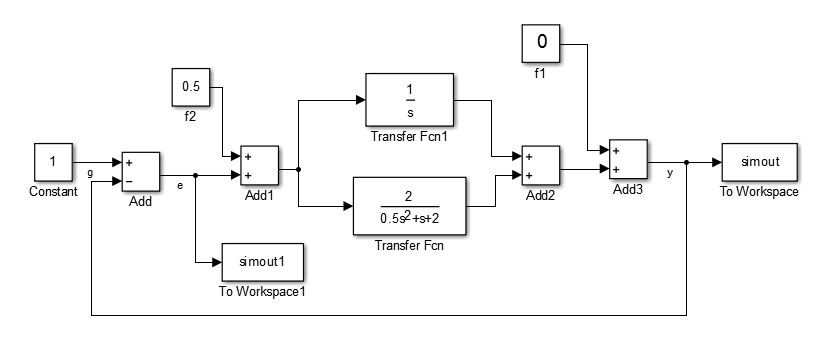
\includegraphics[width=1\linewidth]{3}}
    \caption{Схема моделирования влияния внешних возмущений}
    \label{tree}
\end{figure}

Зададим $f_2(t) = 0, g(t) = 1(t)$

\begin{figure}[h!]
    \center{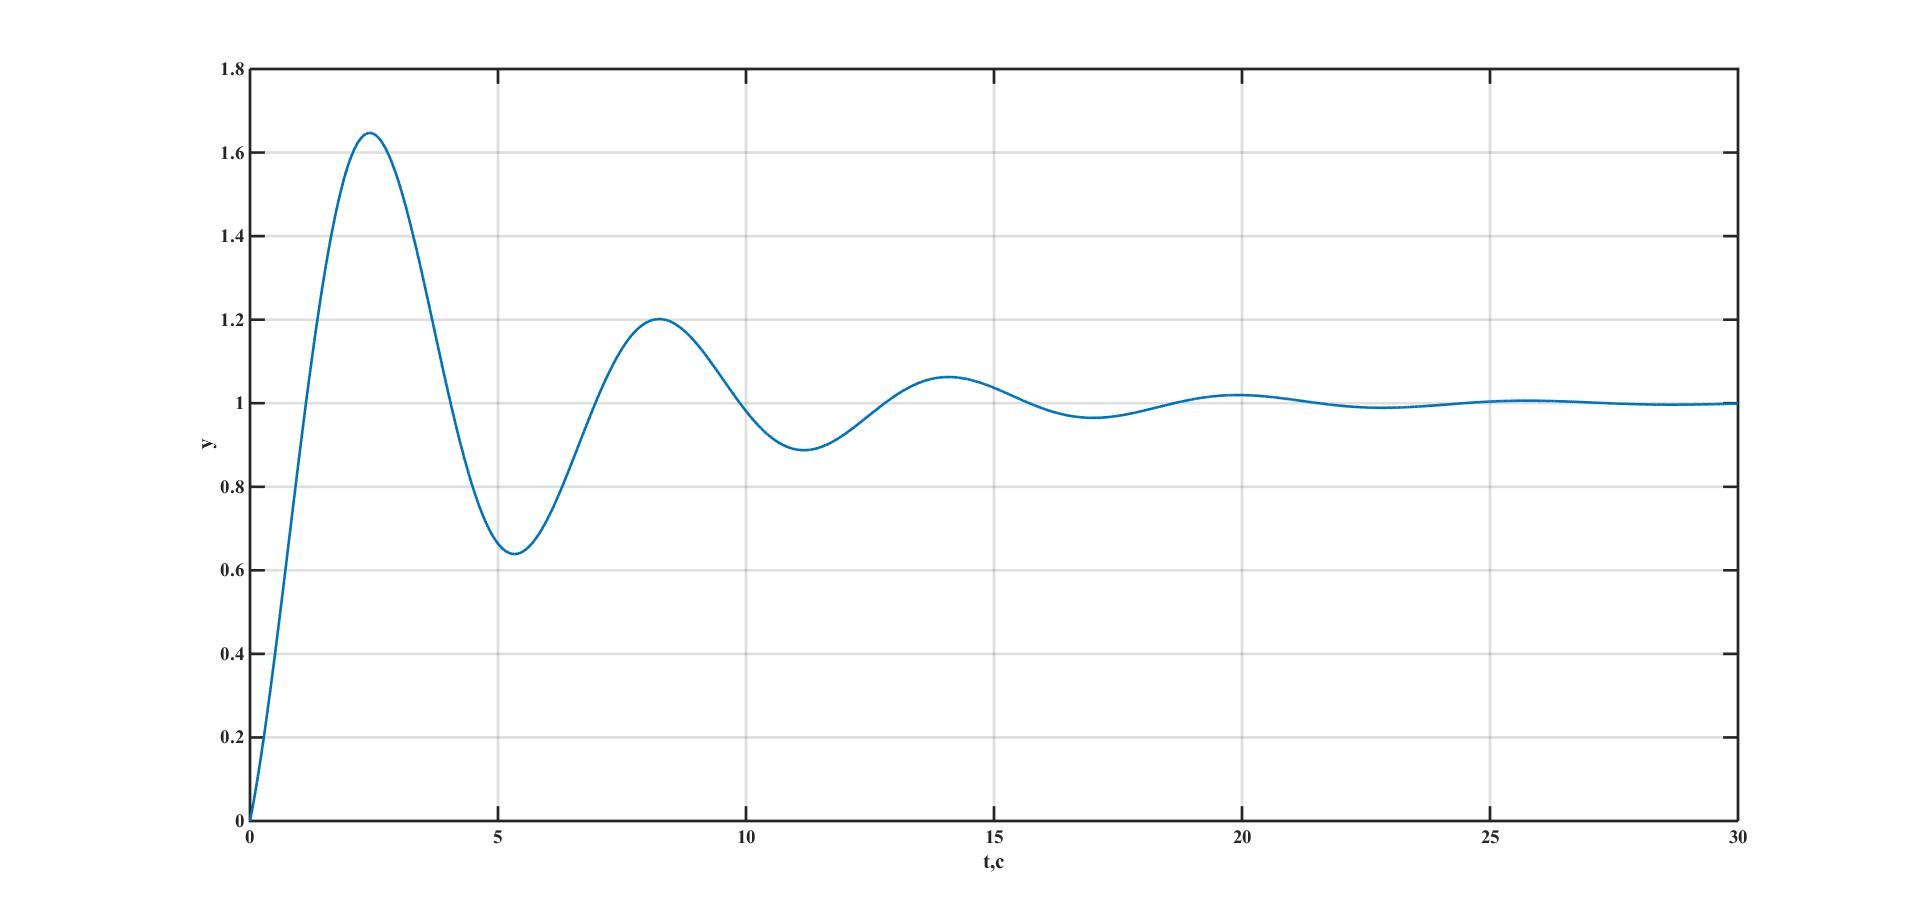
\includegraphics[width=1\linewidth]{3/3f20y}}
    \caption{График переходного процесса при $f_2(t) = 0$}
    \label{two}
\end{figure}

\newpage

\begin{figure}[h!]
    \center{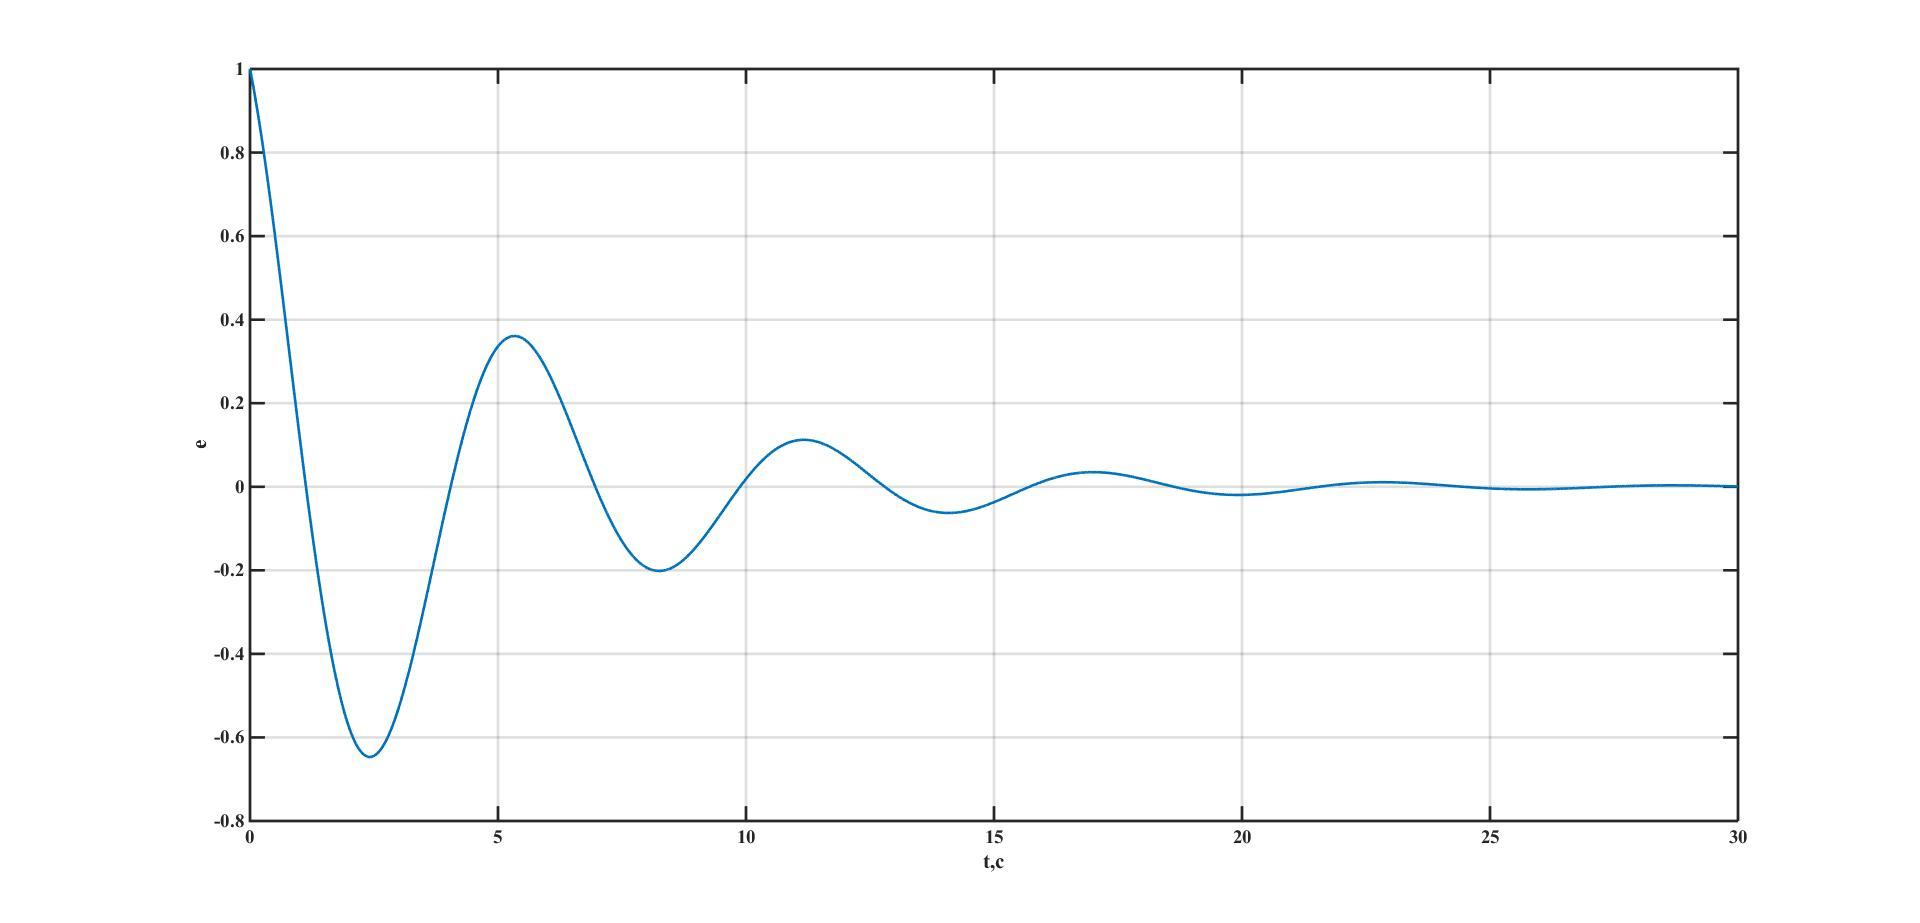
\includegraphics[width=1\linewidth]{3/3f20e}}
    \caption{График ошибки переходного процесса при $f_2(t) = 0$}
    \label{tree}
\end{figure}

Зададим $f_1(t) = 0, g(t) = 1(t)$

\begin{figure}[h!]
    \center{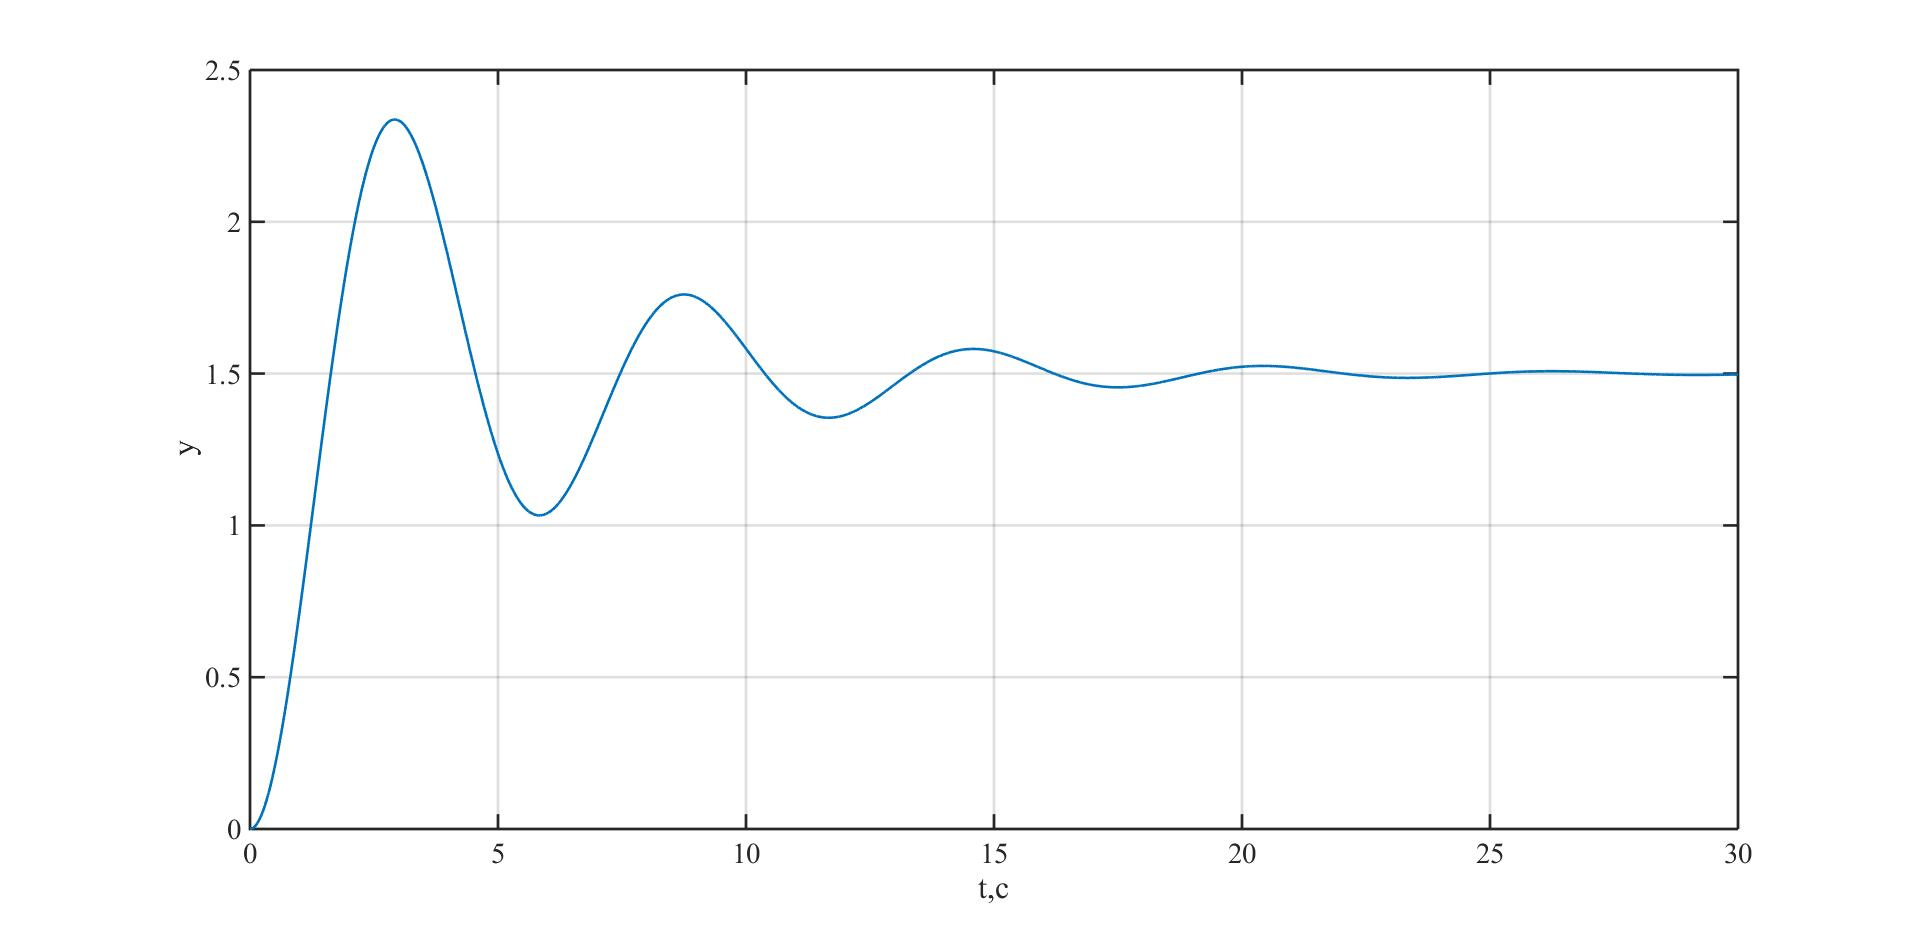
\includegraphics[width=1\linewidth]{3/3f10y}}
    \caption{График переходного процесса при $f_1(t) = 0$}
    \label{two}
\end{figure}
    
\newpage    
    
\begin{figure}[h!]
    \center{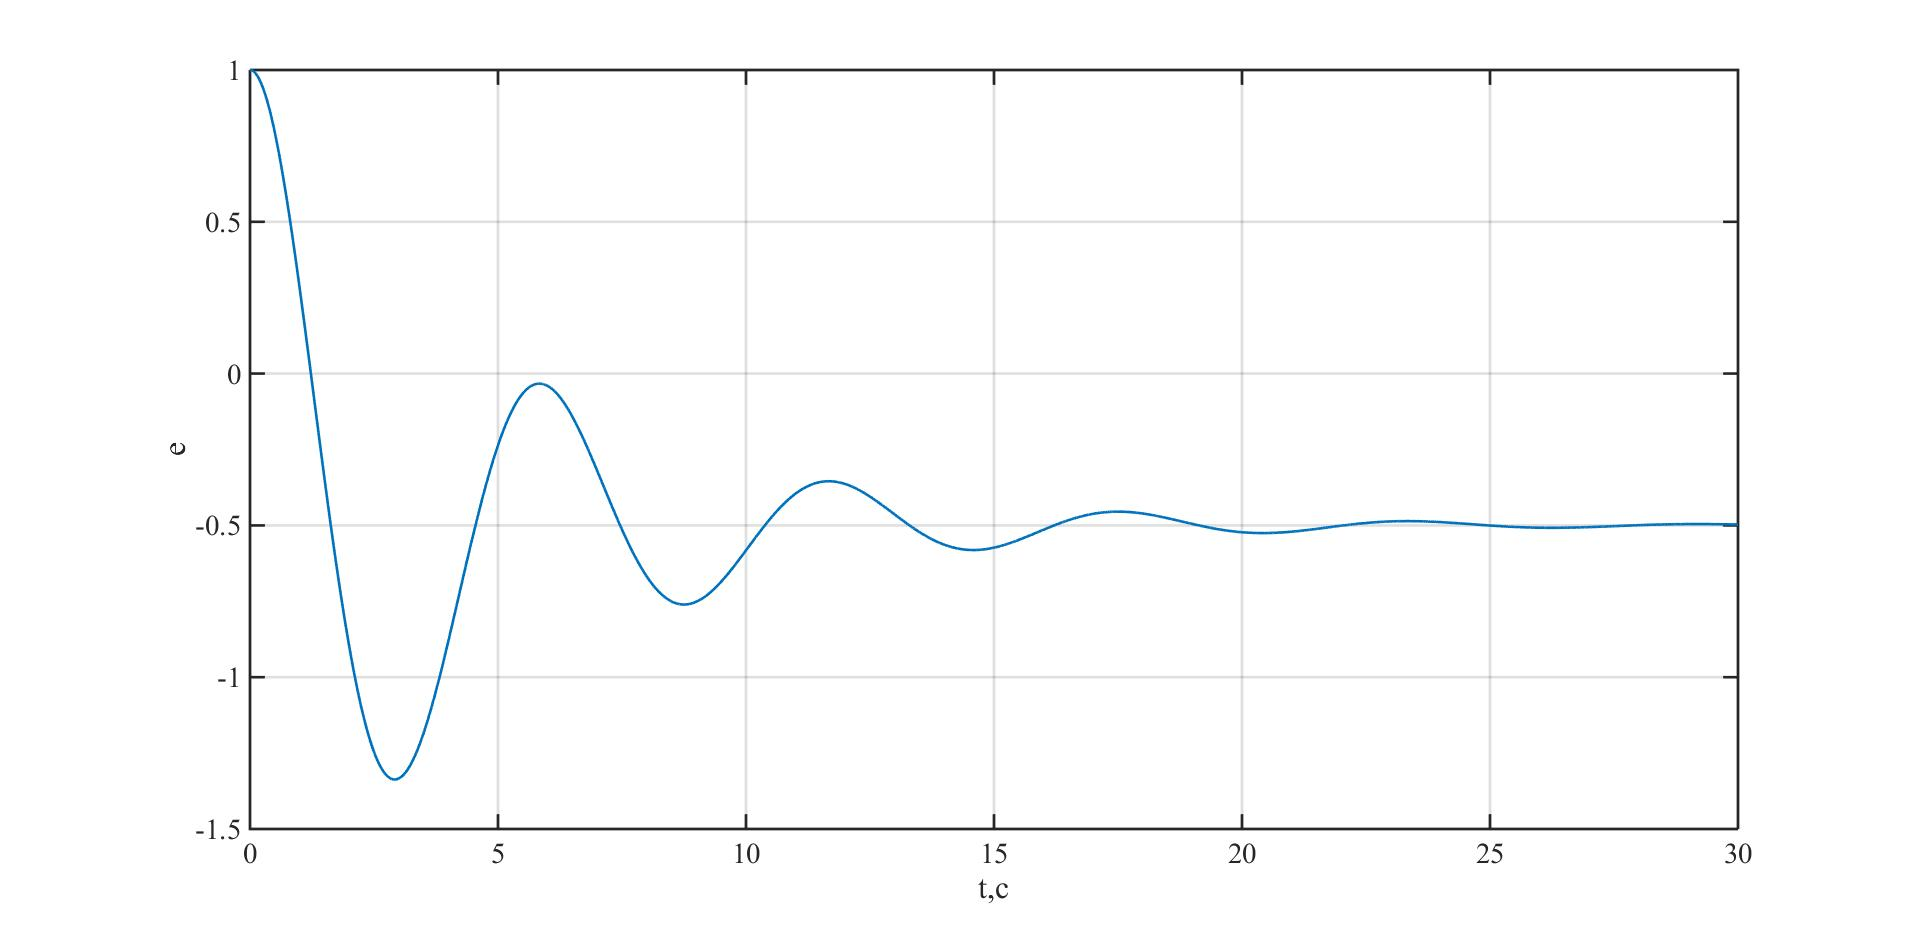
\includegraphics[width=1\linewidth]{3/3f10e}}
    \caption{График ошибки переходного процесса при $f_1(t) = 0$}
    \label{tree}
\end{figure}

Из графика видно, что предельное значение установившейся ошибки $e_y(t)=-0.5$. Это значение подтверждается аналитическим расчетом:
\begin{equation}
	\varepsilon = \lim_{s\to 0}{e(s)} = -f1
\end{equation}

\newpage
\begin{center}
\section{Исследование установившейся ошибки при произвольном входном воздействии}
\end{center}
На рисунке 18 представлена схема моделирования произвольного входного воздействия, также на рисунках 19 и 20 представлены графики переходного процесса и ошибки.

Рассмотрим систему при:\\

$H(s)=1;$ \\

$W(s)=\frac {3} {2.5s+1};$ \\

$g(t)=0.2t^2+sin(0.5t);$

\begin{figure}[h!]
    \center{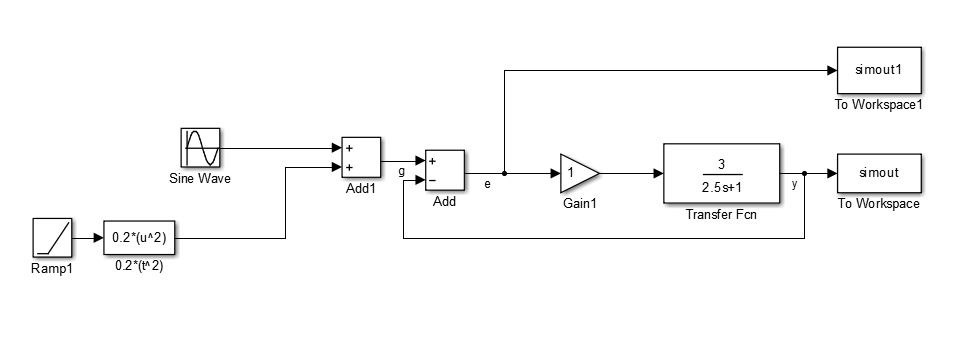
\includegraphics[width=1\linewidth]{4}}
    \caption{Схема моделирования произвольного входного воздействия}
    \label{two}
\end{figure}

\begin{figure}[h!]
    \center{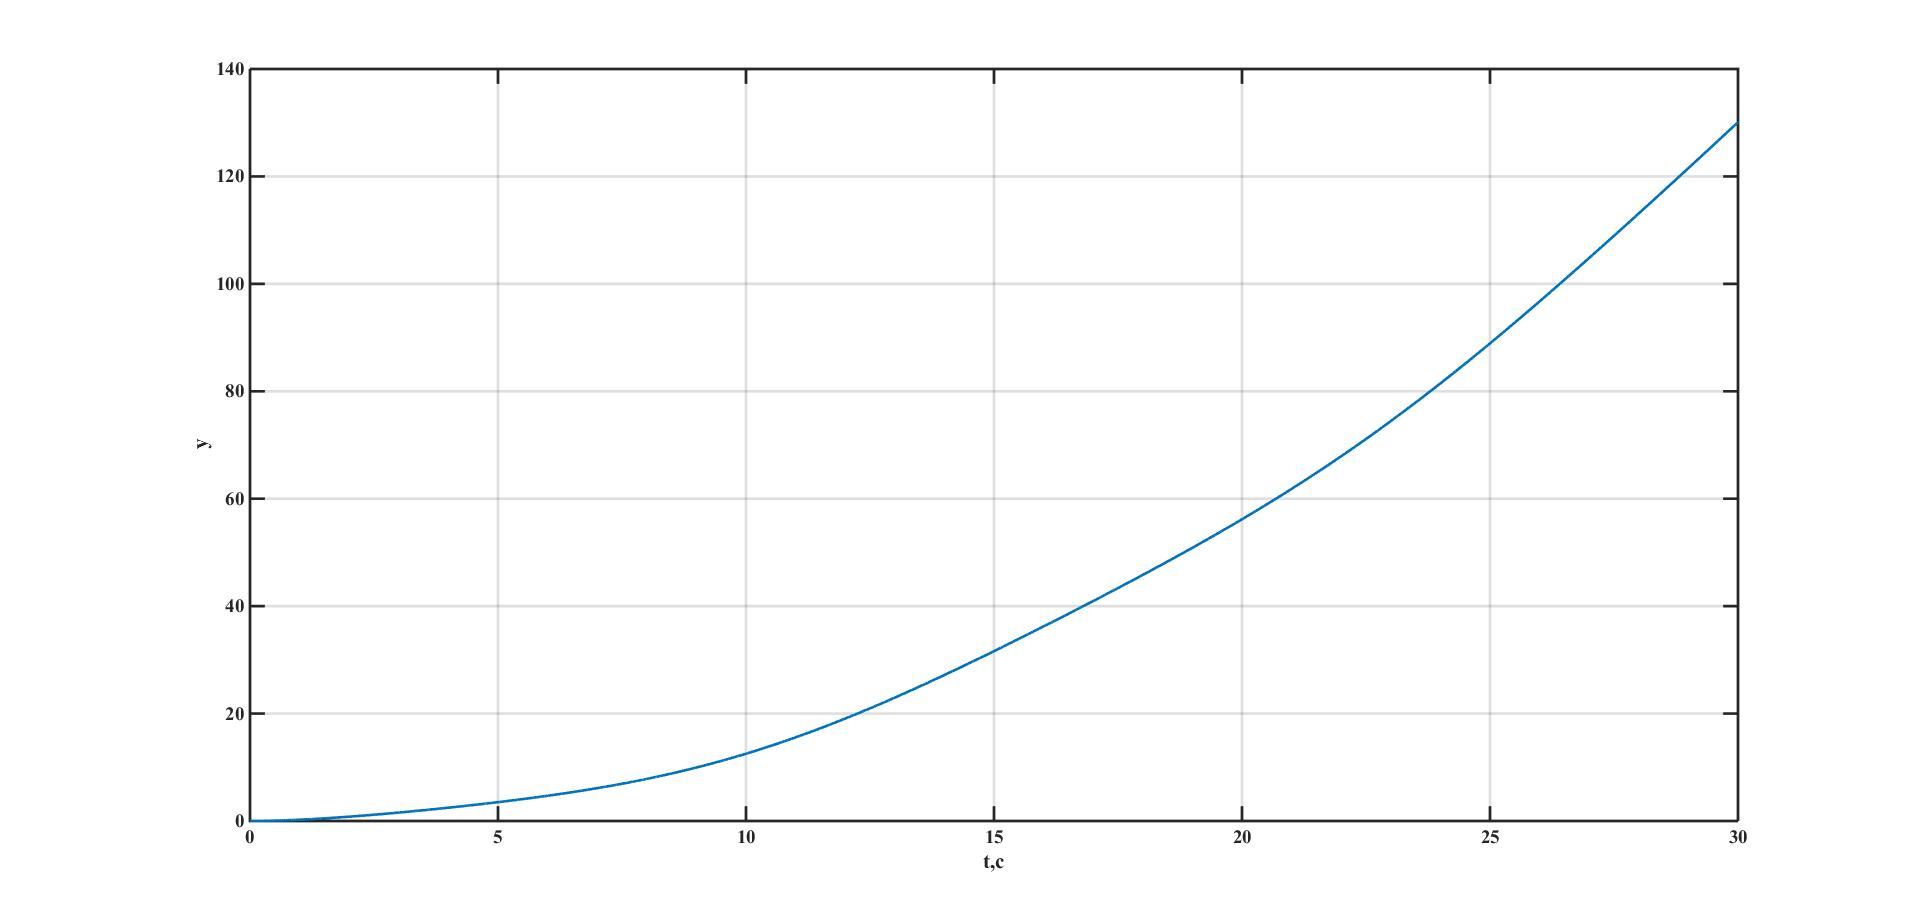
\includegraphics[width=1\linewidth]{4/4_1y}}
    \caption{График переходного процесса}
    \label{two}
\end{figure}

\newpage
    
\begin{figure}[h!]
    \center{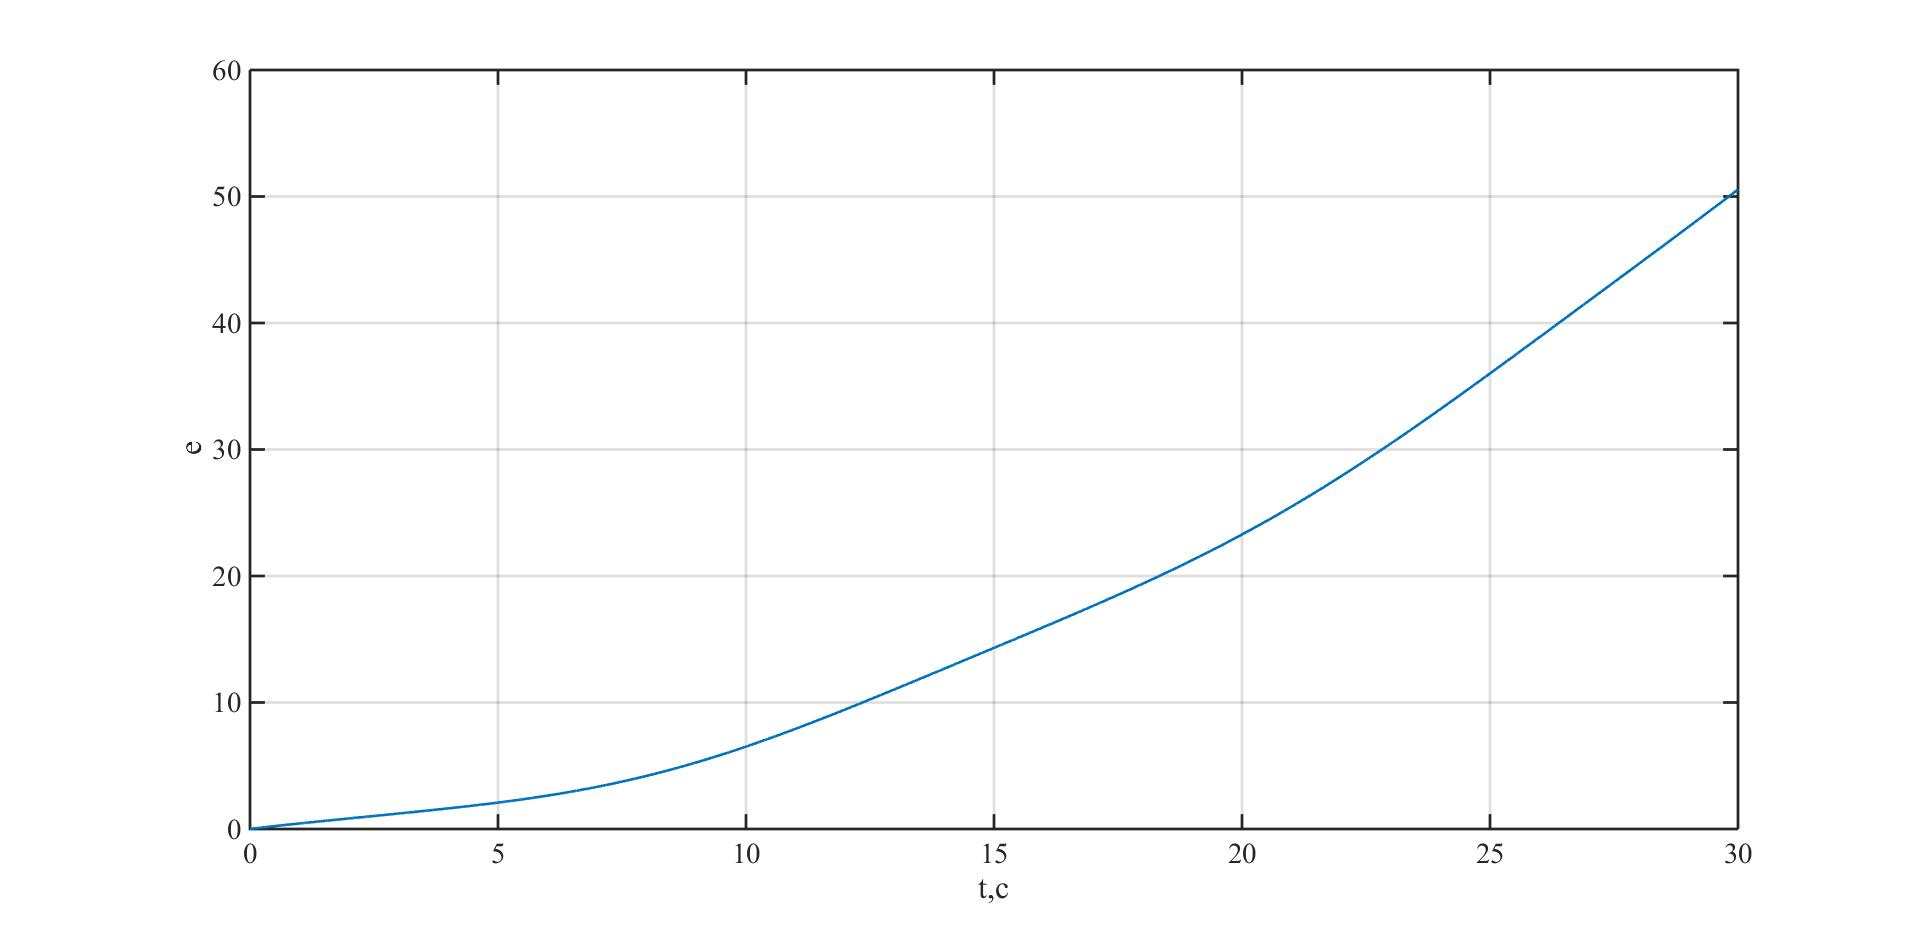
\includegraphics[width=1\linewidth]{4/4_1e}}
    \caption{График ошибки переходного процесса}
    \label{tree}
\end{figure}



$e_y(t)\to\infty$, т.к. СУ с астатизмом нулевого порядка не может отработать линейно нарастающее задающее воздействие.\\

Разложим уравнение ошибки в ряд Тейлора:
$e_y(t)=c_0g(t)+c_1\frac{d}{dt}g(t)+\frac{c_2}{2!}\frac{d^2}{dt^2}g(t)+...$ , где постоянные $c_i$ - коэффициенты ошибок.\\

$\Phi_e(s)=\frac{1}{1+W(s)}$, где W(s) – передаточная функция разомкнутой системы, Фe(s) – передаточная функция замкнутой системы по ошибке слежения (относительно задающего воздействия).\\

	$W(s)=\frac {3} {2.5s+1};$ \\
	
	$\Phi_e(s)=\frac{2.5s+1}{2.5s+4};$ \\
	
	$c_0=\Phi_e(s) | _{s=0} =0.25$ \\
	
	$c_1=\frac{1.2}{2.56}$ \\
	
	$c_2=-\frac{2.4}{4.096}$ \\
	
	$e_y(t)=0.25(0.2t^2+sin(0.5t))+\frac{1.2}{2.56}(0.4t+0.5cos(0.5t))-\frac{2.4}{4.096}(0.4-0.25sin(0.5t))$\\
	
Смоделируем получивийся ряд в матлабе. На 21 представлена схема моделирования функции ошибки, также на рисунке 22 предсавлен получившийся график ошибки.

\newpage 

\begin{figure}[h!]
    \center{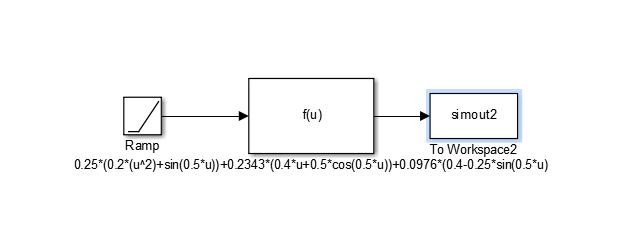
\includegraphics[width=1\linewidth]{teylor}}
    \caption{Схема моделирование. Ряд Тейлора}
    \label{tree}
\end{figure}

\begin{figure}[h]
    \center{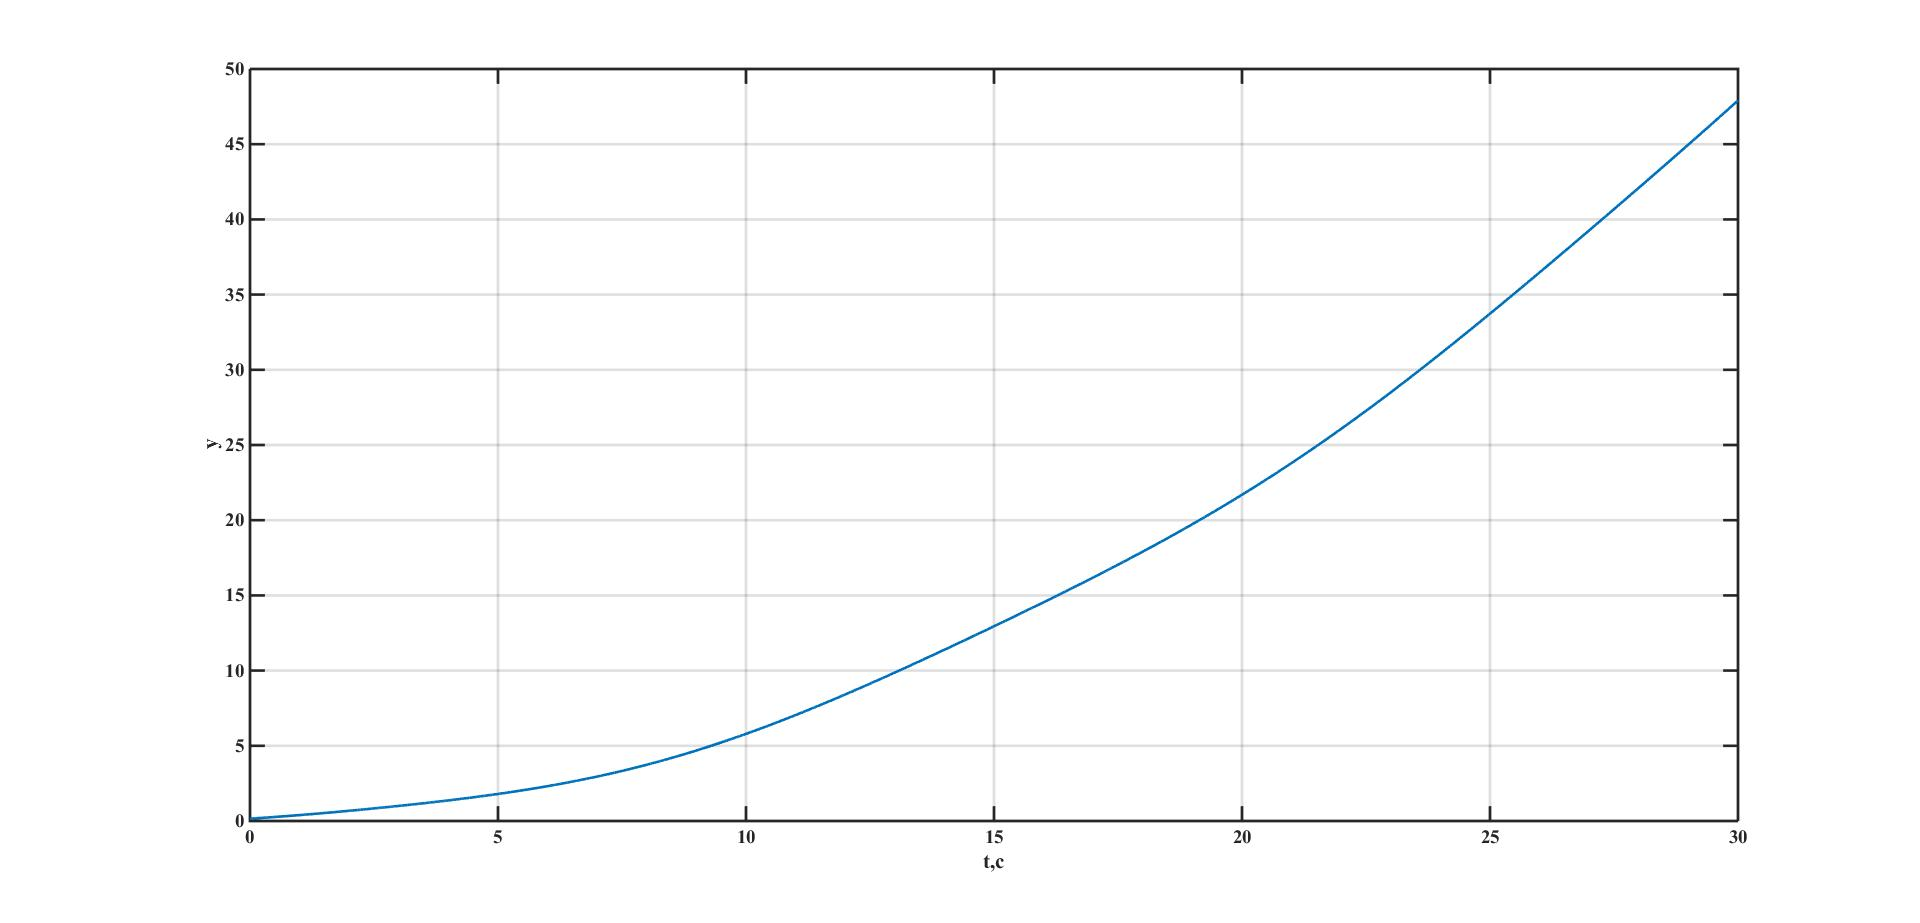
\includegraphics[width=1\linewidth]{4/4_2teylor}}
    \caption{График ошибки переходного процесса}
    \label{tree}
\end{figure}
\newpage
\begin{center}
\section*{Вывод}
\end{center}
 В данной работе мы исследовали передаточные функции с различным остатизмом, при наличии внешних возмущений и без них. Проведенные исследования показали, что, когда сигнал стационарный (g = A), при увеличении коэффициента усиления (К), ошибка стремится к нулю. Также выяснилось, что на наличие или отсутствие установившейся ошибки влияет порядок астатизма: при увеличении порядка астатизма ошибка исчезает, становится равной нулю. Большое влияние оказывают и внешние возмущения: при их наличии входной сигнал увеличивается, и появляется ошибка.

\end{document} % КОНЕЦ ДОКУМЕНТА !

